\section{Introduction}

This chapter evaluates the performance of OmniTune when tasked with
selecting workgroup sizes for SkelCL stencil codes. First I discuss
measurement noise present in the experimental results, and the methods
used to accommodate for it. Then I examine the observed effect that
workgroup size has on the performance of SkelCL stencils. The
effectiveness of each of the autotuning techniques described in the
previous chapters are evaluated using multiple different machine
learning algorithms. The prediction quality of OmniTune is scrutinised
for portability across programs, devices, and datasets.


\subsubsection{Overview of Experimental Results}

The experimental results consist of measured runtimes for a set of
\emph{test cases}, collected using the methodology explained int he
previous chapter. Each test case $\tau_i$ consists of a scenario,
workgroup size pair $\tau_i = (s_i,w_i)$, and is associated with a
\emph{sample} of observed runtimes from multiple runs of the
program. A total of \input{gen/num_runtime_stats} test cases were
evaluated, which represents an exhaustive enumeration of the workgroup
size optimisation space for \input{gen/num_scenarios} scenarios. For
each scenario, runtimes for an average of \input{gen/avg_num_params}
(max \input{gen/max_num_params}) unique workgroup sizes were
measured. The average sample size of runtimes for each test case is
\input{gen/avg_sample_count} (min \input{gen/min_sample_count}, total
\input{gen/num_samples}).


\section{Statistical Soundness}

\begin{figure}
\begin{subfigure}[h]{.32\textwidth}
\centering
\includegraphics{gen/img/runtimes_histogram_1}
\vspace{-1.5em} % Shrink vertical padding
\caption{}
\label{fig:runtimes-histogram-1}
\end{subfigure}
~%
\begin{subfigure}[h]{.32\textwidth}
\centering
\includegraphics{gen/img/runtimes_histogram_2}
\vspace{-1.5em} % Shrink vertical padding
\caption{}
\label{fig:runtimes-histogram-2}
\end{subfigure}
~%
\begin{subfigure}[h]{.32\textwidth}
\centering
\includegraphics{gen/img/runtimes_histogram_3}
\vspace{-1.5em} % Shrink vertical padding
\caption{}
\label{fig:runtimes-histogram-3}
\end{subfigure}
\\
\begin{subfigure}[h]{.32\textwidth}
\centering
\includegraphics{gen/img/runtimes_histogram_4}
\vspace{-1.5em} % Shrink vertical padding
\caption{}
\label{fig:runtimes-histogram-4}
\end{subfigure}
~%
\begin{subfigure}[h]{.32\textwidth}
\centering
\includegraphics{gen/img/runtimes_histogram_5}
\vspace{-1.5em} % Shrink vertical padding
\caption{}
\label{fig:runtimes-histogram-5}
\end{subfigure}
~%
\begin{subfigure}[h]{.32\textwidth}
\centering
\includegraphics{gen/img/runtimes_histogram_6}
\vspace{-1.5em} % Shrink vertical padding
\caption{}
\label{fig:runtimes-histogram-6}
\end{subfigure}
\\
\begin{subfigure}[h]{.32\textwidth}
\centering
\includegraphics{gen/img/runtimes_histogram_7}
\vspace{-1.5em} % Shrink vertical padding
\caption{}
\label{fig:runtimes-histogram-7}
\end{subfigure}
~%
\begin{subfigure}[h]{.32\textwidth}
\centering
\includegraphics{gen/img/runtimes_histogram_8}
\vspace{-1.5em} % Shrink vertical padding
\caption{}
\label{fig:runtimes-histogram-8}
\end{subfigure}
~%
\begin{subfigure}[h]{.32\textwidth}
\centering
\includegraphics{gen/img/runtimes_histogram_9}
\vspace{-1.5em} % Shrink vertical padding
\caption{}
\label{fig:runtimes-histogram-9}
\end{subfigure}

\caption{%
  Distribution of runtime samples for 9 test cases with average
  runtimes between 2--200ms. Each plot contains a 35-bin histogram of
  1000 samples, and a fitted kernel density estimate with bandwidth
  0.3. The sample mean is shown as a vertical dashed line. In some of
  the plots, the distribution of runtimes is bimodal, and skewed to
  the lower end of the runtimes range. The long tail in some
  distributions suggests delays in program execution caused by other
  processes on the test systems. The similarity between sample means
  and peak density estimates suggests that a sufficiently accurate
  estimation of the true mean can be made using the arithmetic mean of
  a large number of observations.%
}
\label{fig:runtime-histograms}
\end{figure}

The complex interaction between processes competing for the finite
resources of a system introduces many sources for noise in program
runtime measurements. Before making any judgements about the relative
performance of optimisation configurations, we must establish the
level of noise present in these measurements. To do this, we evaluate
the distribution of runtimes for a randomly selected 1000 test cases,
recording 1000 1000 runtime observations for each. We can then produce
fine-grained histograms of runtimes for individual test
cases. Figure~\ref{fig:runtime-histograms} shows an example nine of
these, for test cases with mean runtimes between 2--200ms. The plots
show that the distribution of runtimes is not always Gaussian; rather,
it is sometimes bimodal, and generally skewed to the lower end of the
runtime range, with a long ``tail'' to the right. This fits our
intuition that programs have a hard \emph{minimum} runtime enforced by
the time taken to execute the instructions of a program, and that
noise introduced to the system extends this runtime by, for example,
preempting a process so that another may run.

The central limit theorem allows the assumption of an underlying
Gaussian distribution for samples of size $\ge 30$~\cite{Georges2007}.
Given our minimum sample size of \input{gen/min_sample_count}, we can
use 95\% confidence intervals to provide statistical confidence that
the arithmetic mean of observed runtimes with respect to the true
mean. As the number or samples increases, we should expect the size of
the confidence interval to shrink. This is illustrated in
Figure~\ref{fig:ci-trends}, which plots the average size of 95\%
confidence intervals across the 1000 test cases, normalised to their
respective means, as a function of sample size. It shows the
diminishing returns that increasing sample size provides. For example,
increasing the sample count from 10 to 30 results in an approximate
50\% reduction in confidence interval size. Increasing the sample size
from 30 to 50 results in only a 25\% reduction.

\begin{figure}
\centering
\includegraphics{gen/img/ci_trend}
\caption{%
  % FIXME: Check against \input{gen/max_ci} and \input{gen/mean_ci}
  Ratio of confidence interval to mean as a function of sample
  count. Two dashed lines indicate the confidence intervals at the
  minimum (3.7\%) and mean (2.5\%) number of samples used in the
  experimental dataset.%
}
\label{fig:ci-trends}
\end{figure}

By comparing the average confidence interval at different sample
counts against the full experiment results of
\input{gen/num_runtime_stats} test cases, we can assert with 95\%
confidence that the true mean for each test case is within
\input{gen/mean_ci}\% of the sample mean (given the average number of
samples per test case), or \input{gen/max_ci}\% in the worst case (at
the minimum number of samples). This demonstrates a sufficiently low
level of noise that meaningful comparisons can be made between the
performance of different configurations. \FIXME{justify\ldots}


\section{Workgroup Size Optimisation Space}

In this section we explore the impact that the workgroup size
optimisation space has on the performance of stencil codes.

\subsection{Oracle Workgroup Sizes}

\begin{figure}
\centering
\includegraphics{gen/img/num_params_oracle.pdf}
\caption{%
  Accuracy compared to the oracle as a function of the number of
  workgroup sizes used. The best accuracy that can be achieved using a
  single statically chosen workgroup size is
  \protect\input{gen/max_oracle_param_frequency}. Achieving 50\%
  oracle accuracy requires \protect\input{gen/num_wgsizes_50_accuracy}
  distinct workgroup sizes.%
}
\label{fig:oracle-accuracy}
\end{figure}

For each scenario $s$, the oracle workgroup size $\Omega(s)$ is the
workgroup size which resulted in the lowest mean runtime. If the
performance of stencils were independent of workgroup size, we would
expect that the oracle workgroup size would remain constant across all
scenarios $s \in S$. Instead, we find that there are
\input{gen/num_oracle_params} unique oracle workgroup sizes, with
\input{gen/oracle_params_per_scenario_perc}\% of scenarios having a
unique workgroup size. This demonstrates that tuning for optimal
workgroup size is a non-trivial task, requiring
\input{gen/num_wgsizes_50_accuracy} distinct workgroup sizes to
achieve 50\% oracle accuracy (Figure~\ref{fig:oracle-accuracy}).

Figure~\ref{fig:oracle-wgsizes} shows the distribution of oracle
workgroup sizes, demonstrating that there is clearly no ``silver
bullet'' workgroup size which works for all scenarios, and that the
space of oracle workgroup sizes is non linear and complex. The
workgroup size which is most frequently optimal is
\input{gen/max_oracle_param}, which is optimal for
\input{gen/max_oracle_param_frequency} of scenarios. Note that this is
not adequate to use as a baseline for static tuning, as it does not
respect legality constraints, that is
$\input{gen/max_oracle_param_w} \not\in W_{safe}$.


\subsection{Workgroup Size Legality}\label{subsec:legality}

\begin{figure}
  \centering
  \includegraphics{gen/img/max_wgsizes.pdf}
  \vspace{-1.5em} % Shrink vertical padding
  \caption{%
    A subset of the workgroup size optimisation space,
    $w_c \le 100, w_r \le 100$, showing the \emph{coverage} of each
    workgroup size, i.e.\ the ratio of scenarios for which a workgroup
    size satisfies architecture and kernel enforced constraints
    ($W_{\max}(s)$). Workgroup sizes with a coverage of $< 1$ fail to
    satisfy these constraints for one or more scenarios. Only
    workgroup sizes with a coverage of 1 may be used for static
    tuning, which greatly reduces the size of the optimisation space.%
  }
\label{fig:max-wgsizes}
\end{figure}

\begin{figure}
\begin{subfigure}[t]{0.98\textwidth}
\centering
\includegraphics{gen/img/coverage_space.pdf}
\vspace{-1.5em} % Shrink vertical padding
\caption{}
\label{fig:coverage}
\end{subfigure}
\\
\begin{subfigure}[t]{0.98\textwidth}
\centering
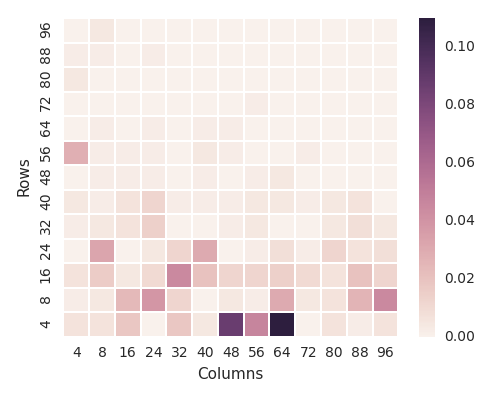
\includegraphics{gen/img/oracle_param_space.pdf}
\vspace{-1.5em} % Shrink vertical padding
\caption{}
\label{fig:oracle-wgsizes}
\end{subfigure}
\caption{%
  Log frequency counts for: (\subref{fig:coverage}) legality, and
  (\subref{fig:oracle-wgsizes}) optimality, for a subset of the
  workgroup size optimisation space, $w_c \le 100, w_r \le 100$.
  Legality frequencies are highest for smaller row and column counts
  (where $w < W_{\max}(s) \forall S$), and $w_c$ and $w_r$ values
  which are multiples of 8. The space of oracle workgroup size
  frequencies is highly irregular and uneven, with a peak frequency of
  $w_{(64 \times 4)}$.%
}
\label{fig:heatmaps}
\end{figure}

As explained in Section~\ref{sec:op-params}, the space of legal
workgroup sizes $W_{legal}(s)$ for a given scenario $s$ comprises all
workgroup sizes which: do not exceed the maximum allowed by the OpenCL
device and kernel $W_{\max}(s)$, and are not refused by the OpenCL
runtime.

\subsubsection{Maximum workgroup sizes}

We define the \emph{coverage} of a workgroup size to be the ratio
$0 \le x \le 1$ between the number of scenarios for which the
workgroup size was less than $W_{\max}(s)$, normalised to the total
number of workgroup sizes. A coverage of 1 implies a workgroup size
which is always legal for all combinations of stencil and
architecture. A workgroup size with a coverage of 0 is never
legal. Figure~\ref{fig:max-wgsizes} plots the coverage of a subset of
the workgroup size optimisation space.

Note that since $W_{\max}(s)$ defines a hard limit for a given $s$, if
statically selecting a workgroup size, one must limit the optimisation
space to the smallest $W_{\max}(s)$ value, i.e.\ only the workgroup
sizes with a coverage of 1. The observed $W_{\max}(s)$ values range
from 256--8192, which results in up to a 97\% reduction in the size of
the optimisation space when $W_{\max}(s) = 8192$, even though only
14\% of scenarios have the minimum value of $W_{\max}(s) = 256$.

% Size of optimisation space for Wmax =  256: 273
% Size of optimisation space for Wmax = 8192: 15925

\subsubsection{Refused Parameters}

\begin{table}
\parbox{.32\linewidth}{
  \centering
  \scriptsize
  \rowcolors{2}{white}{gray!25}
  \input{gen/tab/top_refused_params_1}
}
\hfill
\parbox{.32\linewidth}{
  \centering
  \scriptsize
  \rowcolors{2}{white}{gray!25}
  \input{gen/tab/top_refused_params_2}
}
\hfill
\parbox{.32\linewidth}{
  \centering
  \scriptsize
  \rowcolors{2}{white}{gray!25}
  \input{gen/tab/top_refused_params_3}
}
\caption{%
  The thirty most refused parameters, ranked in descending
  order. There is little correlation between the size of workgroup and the
  likelihood that it is refused, suggesting that the cause of refused
  parameters is not a resource constraint, but a behavioural issue.%
}
\label{tab:top-refused-params}
\end{table}

\begin{figure}
\centering
\begin{subfigure}[h]{.45\textwidth}
  \centering
  \includegraphics{gen/img/refused_params_by_device}
  \caption{}
  \label{fig:refused-params-by-device}
\end{subfigure}
\hfill
\begin{subfigure}[h]{.45\textwidth}
  \centering
  \includegraphics{gen/img/refused_params_by_vendor}
  \caption{}
  \label{fig:refused-params-by-vendor}
\end{subfigure}
\caption{%
  The ratio of test cases with refused workgroup sizes, grouped by:
  (\subref{fig:refused-params-by-device}) OpenCL device ID;\
  (\subref{fig:refused-params-by-vendor}) device vendor ID. Parameters
  were refused most frequently by Intel i5 CPUs, then by
  previous-generation NVIDIA GPUs. No parameters were refused by AMD
  devices.%
}
\label{fig:refused-params-by-dev-vendor}
\end{figure}

In addition to the hard constraints imposed by the maximum workgroup
size, there are also refused parameters, which are workgroup sizes
which are rejected by the OpenCL runtime and do not provide a
functioning program. Of the \input{gen/num_params} unique workgroup
sizes tested, \input{gen/ratio_refused_params}\% were refused in one
or more test cases. An average of
\input{gen/ratio_refused_test_cases}\% of all test cases lead to
refused parameters. For a workgroup size to be refused, it must
satisfy the architectural and program-specific constraints which are
exposed by OpenCL, but still lead to a \texttt{CL\_OUT\_OF\_RESOURCES}
error when the kernel is enqueued. Table~\ref{tab:top-refused-params}
lists the most frequently refused parameters, and the percentage of
test cases for which they were refused. While uncommon, a refused
parameter is an obvious inconvenience to the user, as one would expect
that any workgroup size within the specified maximum should behave
\emph{correctly}, if not efficiently. Figure~\ref{fig:coverage}
visualises the space of legal workgroup sizes by showing the frequency
counts that a workgroup size is legal. Smaller workgroup sizes are
legal most frequently due to the $W_{\max}(s)$ constraints. Beyond
that, workgroup sizes which contain $w_c$ and $w_r$ values which are
multiples of eight are more frequently legal, which is a common width
of SIMD vector operations~\cite{IntelCorporation2012}.

Experimental results suggest that the problem is vendor --- or at
least device --- specific. By grouping the refused test cases by
device and vendor, we see a much greater quantity of refused
parameters for test cases on Intel CPU devices than any other type,
while no workgroup sizes were refused by the AMD
GPU. Figure~\ref{fig:refused-params-by-dev-vendor} shows these
groupings. The exact underlying cause for these refused parameters is
unknown, but can likely by explained by inconsistencies or errors in
specific OpenCL driver implementations.

As these OpenCL implementations are still in active development, it is
anticipated that errors caused by unexpected behaviour will become
more infrequent as the technology matures. For now, it is imperative
that any autotuning system is capable of adapting to these refused
parameters by suggesting alternatives when they occur.

% \TODO{Bug reports\ldots}


\subsection{Baseline Parameter}\label{subsec:baseline}

The baseline parameter $\bar{w}$ is the workgroup size which provides
the best overall performance while being legal for all scenarios. It
is the workgroup size $w \in W_{safe}$ which maximises the output of
the performance function $\bar{p}(w)$. As shown in
Table~\ref{tab:highest-legality}, only a \emph{single} workgroup size
$w_{(4 \times 4)}$ from the set of experimental results is found to
have a legality of 100\%, suggesting that an adaptive approach to
setting workgroup size is necessary not just for the sake of
maximising performance, but also for guaranteeing program correctness.

The utility of the baseline parameter is that it represents the best
performance that can be achieved through static tuning of the
workgroup size parameter. We can evaluate the performance of
suboptimal workgroup sizes by calculating the geometric mean of their
\emph{performance} for a particular scenario $p(s, w)$ across all
scenarios, $\bar{p}(w)$. The geometric mean performance
$\bar{p}(\bar{w})$ of the baseline parameter is
\input{gen/one_r_perf}. Figure~\ref{fig:performance-legality} plots
workgroup size \emph{legality} and \emph{performance}, showing that
there is no clear correlation between the two. In fact, the workgroup
sizes with the highest mean performance are legal for less than 1\% of
all scenarios, which reinforces the claim for autotuning. The
workgroup sizes with the highest legality are listed in
Table~\ref{tab:highest-legality}, and the workgroup sizes with the
highest performance are listed in Table~\ref{tab:highest-performance}.

Figure~\ref{fig:speedups} shows the speedup of the oracle workgroup
size over the baseline parameter $w_{(4 \times 4)}$ for all
scenarios. If we assume that sufficiently pragmatic developer with
enough time would eventually find this static optimal, then this
provides a reasonable comparison for calculating speedups of an
autotuner for workgroup size. Comparing the performance of workgroup
sizes relative to the oracle allows us to calculate upper bounds on
the possible performance which can be expected from autotuning.


\begin{figure}
\centering
\includegraphics{gen/img/params_summary.pdf}
\caption{%
  Average legality and performance of all workgroup sizes. Clearly,
  the relationship between legality and performance is not
  linear. Distinct vertical ``bands'' appear between regions of
  legality caused by the different $W_{\max}(s)$ values of
  devices. The irregular jitter between these vertical bands is caused
  by refused parameters.%
}
\label{fig:performance-legality}
\end{figure}


\begin{table}
  \parbox{.45\linewidth}{
    \centering
    \scriptsize
    \rowcolors{2}{white}{gray!25}
    \input{gen/tab/top_params_coverage}
    \caption{%
      The 25 workgroup sizes with the greatest legality.%
    }
\label{tab:highest-legality}
  }
  \hfill
  \parbox{.45\linewidth}{
    \centering
    \scriptsize
    \rowcolors{2}{white}{gray!25}
    \input{gen/tab/top_params_perf}
    \caption{%
      The 25 workgroup sizes with the greatest mean
      performance.%
    }
\label{tab:highest-performance}
  }
\end{table}


\subsection{Performance Upper Bounds}

\begin{figure}
  \includegraphics{gen/img/max_speedups}
  \caption{%
    Speedup of oracle workgroup size over: the worst performing
    workgroup size for each scenario (\emph{Max}), the statically
    chosen workgroup size that provides the best overall performance
    ($w_{(4 \times 4)}$), and the human expert selected parameter
    ($w_{(32 \times 4)}$). Note that the human expert parameter is not
    legal for all scenarios.%
  }
\label{fig:speedups}
\end{figure}

For a given scenario $s$, the ratio of the workgroups sizes from
$W_{legal}(s)$ which provide the longest and shortest mean runtimes is
used to calculate an upper bound for the possible performance
influence of workgroup size:

\begin{equation}
r_{max}(s) = r(s, \argmax_{w \in W_{legal}(s)} t(s,w), \Omega(s))
\end{equation}

When applied to each scenario $s \in S$ of the experimental results,
we find the average of performance upper bounds to be
$\input{gen/avg_possible_speedup}\times$ (min
$\input{gen/min_possible_speedup}\times$, max
$\input{gen/max_possible_speedup}\times$). This demonstrates the
importance of tuning stencil workgroup sizes --- if chosen
incorrectly, the runtime of stencil programs can be extended by up to
$\input{gen/max_possible_speedup}\times$. Note too that for 5 of the
scenarios, the speedup of the best over worst workgroup sizes is
$\le 5\%$.
% TODO: t-test for this!
For these scenarios, there is little benefit to autotuning; however,
this represents only 1.1\% of the tested scenarios. For 50\% of the
scenarios, the speedup of the best over worst workgroup sizes is
$\ge 6.19\times$.


\subsection{Human Expert}

% SCENARIOS IN WHICH 32x4 WAS NOT LEGAL:
%
% sqlite> select distinct name,kernels.north,kernels.south,kernels.east,kernels.west,device,dataset,name from runtime_stats left join scenarios on runtime_stats.scenario=scenarios.id left join kernel_names on scenarios.kernel=kernel_names.id left join kernels on scenarios.kernel=kernels.id where scenario NOT IN (select scenario from runtime_stats where params="32x4");
% name        north       south       east        west        device                                     dataset                name
% ----------  ----------  ----------  ----------  ----------  -----------------------------------------  ---------------------  ----------
% complex     30          30          30          30          1xIntel(R) Core(TM) i5-4570 CPU @ 3.20GHz  1024.1024.float.float  complex
% simple      0           0           0           0           1xIntel(R) Core(TM) i5-2430M CPU @ 2.40GH  1024.1024.float.float  simple
% complex     30          30          30          30          1xIntel(R) Core(TM) i5-2430M CPU @ 2.40GH  2048.2048.float.float  complex
% complex     1           10          30          30          1xIntel(R) Core(TM) i5-4570 CPU @ 3.20GHz  512.512.float.float    complex
% simple      30          30          30          30          1xIntel(R) Core(TM) i5-2430M CPU @ 2.40GH  512.512.float.float    simple
% complex     30          30          30          30          1xGeForce GTX 690                          512.512.float.float    complex
% simple      20          10          20          10          1xIntel(R) Core(TM) i5-2430M CPU @ 2.40GH  4096.4096.float.float  simple
% simple      1           10          30          30          1xIntel(R) Core(TM) i5-2430M CPU @ 2.40GH  2048.2048.float.float  simple
% complex     30          30          30          30          1xGeForce GTX 690                          1024.1024.float.float  complex
% complex     1           10          30          30          1xIntel(R) Core(TM) i5-2430M CPU @ 2.40GH  2048.2048.float.float  complex
% simple      30          30          30          30          1xGeForce GTX 690                          512.512.float.float    simple

In the original implementation of the SkelCL stencil
skeleton~\cite{Breuer2013}, \citeauthor{Breuer2013} selected a
workgroup size of $w_{(32 \times 4)}$ in an evaluation of 4 stencil
operations on a Tesla S1070 system. We can use this as an additional
parameter to compare the relative performance of workgroup sizes
against. However, the $w_{(32 \times 4)}$ workgroup size is invalid
for 2.6\% of scenarios, as it is refused in 11 test cases. By device,
those are: 3 on the GTX 690, 6 on the i5-2430M, and 2 on the i5-4570.
For the scenarios where $w_{(32 \times 4)}$ \emph{is} legal, the human
expert chosen workgroup size achieves an impressive geometric mean of
79.2\% of the oracle performance. The average speedup of oracle
workgroup sizes over the workgroup size selected by a human expert is
$1.37\times$ (min $1.0\times$, max $5.17\times$). Since the workgroup
size selected by the human expert is not legal for all scenarios, we
will examine the effectiveness of heuristics for tuning workgroup
size.


\subsection{Heuristics}\label{subsec:heuristics}

In this section we will consider the effectiveness of instead
selecting workgroup size using two types of heuristics. The first,
using the maximum workgroup size returned by the OpenCL device and
kernel APIs to select the workgroup size adaptively. The second, using
per-device heuristics, in which the workgroup size is selected based
on the specific architecture that a stencil is operating on.

\subsubsection{Using maximum legal size}

A common approach taken by OpenCL developers is to set the workgroup
size for a kernel based on the maximum legal workgroup size queried
from the OpenCL APIs. For example, to use the square root of the
maximum to set the number of columns and rows for a 2D NDRange. To
consider the effectiveness of this approach, we group the workgroup
size performances based on the ratio of the maximum allowed for each
scenario. We can also perform this for each of the two components ---
rows and columns --- of the stencil workgroup
size.

Figure~\ref{fig:performance-wgsizes} the distribution of runtimes when
grouped this way, demonstrating that the performance of (legal)
workgroup sizes are not correlated with the maximum workgroup sizes
$W_{\max}(s)$. However, when considering individual components, we
observe that the best median workgroup size performances are achieved
with a number of columns that is between 10\% and 20\% of the maximum,
and a number of rows that is between 0\% and 10\% of the maximum.

\subsubsection{Per-device workgroup sizes}

\begin{table}
\scriptsize
\centering
\rowcolors{2}{white}{gray!25}
\input{gen/tab/heuristics-dev}
\caption{%
  Selecting workgroup size using a per-device heuristic. The mode
  optimal workgroup size for each device type $\bar{w}$ is evaluated
  based on legality, and relative performance to the oracle (minimum
  and average) when legal.%
}
\label{tab:heuristic-dev}
\end{table}

One possible approach to selecting workgroup size is to tune
particular values for each execution device. While this approach
scales poorly and is impractically expensive for widespread use, it is
sometimes adopted for cases with particularly high requirements for
performance on a single platform, so it produces an interesting
contrast to evaluating a machine learning approach.

Figure~\ref{fig:performances} shows the performance of workgroup sizes
relative to the oracle across scenarios grouped by: kernel, device,
and dataset. When grouped like this, a number of observations can
made. First is that not all of the kernels are sensitive to tuning
workgroup size to the same degree. The \emph{sobel} kernel has the
lowest median performance, indicating that it is the most profitable
to tune, while the \emph{threshold} kernel is the least
profitable. Similarly, the Intel i7-3820 is far less amenable to
tuning than the other devices, while the Intel i5-4570 is the most
sensitive to the workgroup size parameter. Such variances in the
distributions of workgroup sizes suggest that properties underlying
the architecture, kernel, and dataset all contribute towards the
proper selection of workgroup size.

To test the performance of a per-device heuristic for selecting
workgroup size, we group the scenarios by device, and compare the
relative performance of all workgroup sizes for each group of
scenarios. The most frequently optimal workgroup size $\bar{w}$ for
each device is selected, and the legality and performance of each
scenario using that workgroup size is evaluated.
Table~\ref{tab:heuristic-dev} shows the results of this evaluation.
The GTX 690 and GTX TITAN share the same $\bar{w}_{(64 \times 4)}$
value, while every other device has a unique optimum. The general case
performance of these per-device parameters is very good, although
legality is only assured for the GTX TITAN and AMD 7970 (which did not
refuse any parameters). However, the worst case performance of
per-device workgroup sizes is poor for all except the i7-3820 (which
is least sensitive to tuning), suggesting that device alone is not
capable to reliably inform the choice of workgroup size.


\begin{figure}
\begin{subfigure}[h]{\textwidth}
\centering
\includegraphics{gen/img/performance_max_wgsize}
\vspace{-1.5em} % Shrink vertical padding
\caption{}
\label{fig:performance-max-wgsize}
\end{subfigure}
\\
\begin{subfigure}[h]{.48\textwidth}
\centering
\includegraphics{gen/img/performance_max_c}
\vspace{-1.5em} % Shrink vertical padding
\caption{}
\label{fig:performance-wg-c}
\end{subfigure}
~%
\begin{subfigure}[h]{.48\textwidth}
\centering
\includegraphics{gen/img/performance_max_r}
\vspace{-1.5em} % Shrink vertical padding
\caption{}
\label{fig:performance-wg-r}
\end{subfigure}

\caption{%
  Comparing workgroup performance relative to the oracle as function
  of: (\subref{fig:performance-max-wgsize})~maximum legal size,
  (\subref{fig:performance-wg-c})~number of columns, and
  (\subref{fig:performance-wg-r})~ number of rows.%
}
\label{fig:performance-wgsizes}
\end{figure}
\newpage
\begin{figure}t
\begin{subfigure}[h]{\textwidth}
\centering
\includegraphics{gen/img/performance_kernels.pdf}
\vspace{-1.5em} % Shrink vertical padding
\caption{Kernels}
\label{fig:performance-kernels}
\end{subfigure}
\\
\begin{subfigure}[h]{.48\textwidth}
\centering
\includegraphics{gen/img/performance_devices.pdf}
\vspace{-1.5em} % Shrink vertical padding
\caption{Devices}
\label{fig:performance-devices}
\end{subfigure}
~%
\begin{subfigure}[h]{.48\textwidth}
\centering
\includegraphics{gen/img/performance_datasets.pdf}
\vspace{-1.5em} % Shrink vertical padding
\caption{Datasets}
\label{fig:performance-datasets}
\end{subfigure}

\caption{%
  Performance relative to the oracle of workgroup sizes across all
  test cases, grouped by: (\subref{fig:performance-kernels})~kernels,
  (\subref{fig:performance-devices})~devices, and
  (\subref{fig:performance-datasets})~datasets.%
}
\label{fig:performances}
\end{figure}


\subsection{Summary}

In this section we have explored the performance impact of the
workgroup size optimisation space. By comparing the relative
performance of an average of \input{gen/avg_num_params} workgroup
sizes across \input{gen/num_scenarios} scenarios, the following
conclusions can be drawn:

\begin{enumerate}
\item The performance of a workgroup size for a particular scenario
  depends properties of the hardware, software, and dataset.
\item The performance gap between the best and workgroup sizes for a
  particular combination of hardware, software, and dataset is up to
  $\input{gen/max_possible_speedup}\times$.
\item Not all workgroup sizes are legal, and the space of legal
  workgroup sizes cannot statically be determined. Adaptive tuning of
  workgroup size is required to ensure reliable performance.
\item Differing scenarios have wildly different optimal workgroup
  sizes, and the best performance can be achieved using static tuning
  is optimal for only \input{gen/max_oracle_param_frequency} of
  workloads.
\end{enumerate}

% I believe this presents a compelling case for the development of an
% autotuner which can select the optimal workgroup size at runtime.

In the following section, we will evaluate the performance of OmniTune
for selecting workgroup sizes.


\section{Predicting Optimal Workgroup Sizes}


To evaluate the performance of a classifier, a subset of scenarios
$S_{training} \subset S$ are labelled with the workgroup size which
gave the best performance for each. The classifier is trained on this
labelled training data, and tested using a set of unseen scenarios
$S_{testing} = S - S_{training}$. The performance of each predicted
oracle workgroup size is compared against the true oracles for that
seTODO{What is the average speedup achieved using different
  classifiers?}

\TODO{What percentage of the maximum performance do the classifiers
  achieve?}

\begin{figure}
\centering
\includegraphics{gen/img/classification-xval.pdf}
\caption{%
  Classification performance using cross-validation.%
}
\end{figure}

\begin{figure}
\centering
\includegraphics{gen/img/classification-xval-random.pdf}
\caption{%
  Per-instance performances of classification using cross-validation
  and the ``random'' error handler.%
}
\end{figure}


\TODO{Rank eigenvectors of PCA on features.}

\TODO{Evaluate the effectiveness of training with synthetic
  benchmarks.}

\subsection{Selection of Features}

\TODO{How does the selection of features affect performance? Show a
  plot of performance vs number of features.}


\subsection{Effectiveness of Synthetic Benchmarks}

\TODO{How well does classification perform when trained solely on
  synthetic benchmarks, and tested soley on real benchmarks?}

\TODO{Repeat the above, but with incremtally fewere benchmarks.}


\subsection{Autotuning Overheads}

\TODO{What is the costs of auto-tuning?}

\TODO{How many iterations do we need to do before we ``break even''?}

\subsection{Summary}


\section{Predicting Stencil Runtime}

\begin{enumerate}
\item How accurately does it predict the runtime of a stencil?
\item What is the relationship between \emph{classification} accuracy,
  and the accuracy of predicted runtimes? Does it really matter if the
  predicted runtime is inaccurate?
\end{enumerate}

\begin{figure}
\centering
\includegraphics{gen/img/runtime-regression-xval.pdf}
\caption{%
  Performance of regressors at predicting program runtime.%
}
\end{figure}

\subsection{Summary}


\section{Predicting Relative Performance}

\subsection{Summary}



% \section{Comparison with hand tuned implementations}

% \TODO{%
%   Compare performance against some hand-crafted implementation of one
%   of the real benchmarks.%
% }


\section{Summary}

% \begin{table}
% \scriptsize
% \input{\DataDir/tab/xval.tex}
% \caption{Results of 10 fold cross-validation.}
% \end{table}

% \begin{table}
% \scriptsize
% \input{\DataDir/tab/synthetic_real.tex}
% \caption{Results of training using synthetic benchmarks and testing on
%   real.}
% \end{table}
